\chapter{Linear Regression}
\label{chapter:linear}
\begin{center}
  {\Large\textit{The best material model of a cat is another, or preferably the same, cat.\\ \vspace{0.1in} - Norbert Wiener}}
\end{center}
\vspace{0.2in}

\section{Introduction}
Linear regression is probably the most fundamental statistical model.  Both because of its simplicity, interpretability, range of applicability, and the fact that more complex models can be studied in ``linearized'' forms where they reduce to linear regression.  Through understanding of mathematical details we hope to convey the following message:  The ability of your model to facilitate prediction and/or inference is only as good as your model's ability to describe the real-world interactions.  

Suppose we wish to model height as a function of age.  A completely ridiculous model would be:
\begin{align*}
  height &= w_0  + w_1 \cdot age.
\end{align*}
The constants $w_0$ and $w_1$ are the same for every individual.  This model is unrealistic since it implies first that your age completely determines your height, and second, because it implies this relationship is linear.  Assuming a deterministic universe, the real model could be written (with $y$ denoting height and $x$ denoting age) $y = f(x, z)$ where $z$ represents a (huge) set of variables (e.g. sex, age, or every subatomic particle in the universe).  Assuming differentiability with respect to $x$ this can be linearized around some point $(\bar x, \bar z)$ to produce
\begin{align*}
    y &= f(\bar x, \bar z) + (x-\bar x)\frac{\p f}{\p x}(\bar x, \bar z) + R(x, z).
\end{align*}
This relation is ``almost linear'' if the remainder $R$ is small.  This would be the case e.g. if the effects of $z$ were small and $x$ was always close to $\bar x$.
In any case, with no assumptions, we can write
\begin{align}
  \begin{split}
    y &= w_0 + w_1 x + (f(x,z) - w_0 - w_1 x)\\
    &= w_0 + w_1 x + \eps(x,z),
  \end{split}
  \label{linear:align:error-decomposition}
\end{align}
where the error $\eps(x,z)$ accounts for effects not given by the first two terms.  

Notice that so far we have not introduced any probabilistic concepts.  There is a problem however in that we cannot possibly hope to write down the function $\eps(x,z)$.  To quantify this uncertainty, we model it as a random variable.  This is reasonable under the following viewpoint.  Suppose we select individuals from the population at large by some random sampling process.  Then, for each fixed age $x$, the probability that $z \in A$ will be given by the fraction of the total population with $(x, z) = \{x\}\times A$.  What is more difficult is to select the distribution of $\eps$.  Once again, fixing $x$, we are left with many random effects on height (the effects of the many variables in $z$).  If these effects are all small, then a central limit result allows us to adequately approximate $\eps(z\g x) \approx \calN(\mu(x), \sigma^2(x))$.  A more likely scenario would be that the sex of the individual has a huge effect and $\eps(z)$ would exhibit (at least) two distinct modes.  Suppose however that we fix sex at Female (also fixing ethnicity, parents height, nutrition, and more\ldots), then we will be left with a number of small effects that can likely be modeled as normal, we then have $\eps(z\g x) \approx\calN(\mu(x), \sigma^2(x))$.  The dependence of the noise on our covariate $x$ is still impossible to remove, e.g. $\sigma(x)$ should be much larger for teenagers than adults.  
So what to do?  There are methods for dealing with non-normality and dependence of $\eps$ on $x$ (e.g. generalized linear models and models dealing with heteroscedasticity).  What is most commonly done (at least as a first hack) is to add more explicitly modeled variables (e.g. nonlinear functions of $x$) and to segment the data (e.g. to build a separate model for women and men).  Our approach to teaching is to show exactly how these problems show up numerically, and allow the reader to decide what should be done.

\begin{digression*}[Inference and Prediction]
  Statistical inference is a general term for drawing conclusions from data.  This could be the (possibly rejecting) the hypothesis that some set of variables $(x,y)$ are independent, or more subtly, inferring a causal relationship from $x$ to $y$.  Prediction is more specific and refers to the ability to predict $y$, when given the information $x$.  
For example, suppose we model 
  \begin{align*}
    &\log\frac{\rmP[\mbox{Cancer}]}{\rmP[\mbox{No-Cancer}]} \\
    \quad &= w_0 + w_1\cdot \mbox{Age} + w_2\cdot\mbox{cardiovascular-health} + w_3\cdot \mbox{is-smoker},
  \end{align*}
Since smoking is associated with a decrease in cardiovascular health, it is possible that a number of different $(w_2, w_3)$ combinations could fit the data equally well.  A typical inference question would be ``can we reject the null hypothesis that smoking does not effect the probability of getting cancer.''  In this case, we should worry whether or not $w_3$ truly captures the effect of smoking.  In the case of prediction, any combination of $(w_2, w_3)$ that predicts well is acceptable.  In this sense, the models used for prediction can often be more ``blunt.''  

In this text we phrase most of our examples as prediction problems since this avoids adding the messy details of proper statistical interpretation.
\end{digression*}

If we observe the age of $N$ individuals we can group the data and write this as:
\begin{align*}
  \left( 
  \begin{matrix}
    Y_1\\\vdots\\Y_N
  \end{matrix}
  \right) &= \left( 
  \begin{matrix}
    1 & X_{12}\\
    \vdots & \\
    1 & X_{N2}
  \end{matrix}
  \right) \left( 
  \begin{matrix}
    w_0\\w_1
  \end{matrix}
  \right) 
  + \left( 
  \begin{matrix}
    E_1\\\vdots\\E_N
  \end{matrix}
  \right)
\end{align*}
where $X_{12}$ is the age of the first individual, and $X_{22}$ the age of the second, and so on.

More generally, we will model each response $Y_n$ as depending on a number of covariates $(X_{n0},\cdots,X_{nK})$, where, by convention we select $X_{n0} \equiv1$.  This gives the matrix equations of linear regression
\begin{align}
  Y &= X w + E.
  \label{linear:align:matrix-equation}
\end{align}

\section{Coefficient Estimation: Bayesian Formulation}
\label{linear:section:bayesian}
Consider \eqref{linear:align:matrix-equation}.  The error term $E$ is meant to represent un-modelable aspects of the $x/y$ relationship.  The part that we do model is determined by $w$.  It is $w$ then that becomes the primary focus of our analysis (although we emphasize that a decent error model is important).  To quantify our uncertainty in $w$ we can take the Bayesian viewpoint that $w$ is a random variable.  This leads to insight about how uncertainty in $w$ changes along with the data and model.

\subsection{Generic setup}
\label{linear:subsection:generic}
Assume we have performed $N$ experiments, where in each one we have taken measurements of $K$ covariates $(X_{n1},\cdots,X_{nK})$.  We then seek characterize the \emph{posterior} density\footnote{For simplicity we always assume our distributions are absolutely continuous with respect to Lebesgue measure, giving rise to density functions.} function $p(w\g X,Y)$.  This is the probability density function (pdf) of our unknown coefficients $w$, conditioned on (given that we know) the measurements $X$, $Y$.  We will always take the viewpoint that $X$ is a fixed set of deterministic measurements, and we therefore will no longer explicitly condition on $X$.  Due to Bayes rule this can be decomposed as:
\begin{align}
  p(w\g Y) &= \frac{p(w)p(Y\g w)}{p(Y)}.
  \label{linear:align:bayes}
\end{align}
This posterior will be used to quantify our uncertainty about the coefficients after measuring our training data.  Moreover, given a new input $x$, we can characterize our uncertainty in the response $y$ by
\begin{align}
  \begin{split}
    p(y\g x, Y) &= \int p(y,w\g x, Y)\dw  = \int p(y\g w, x)p(w\g Y)\dw.
  \end{split}
  \label{linear:align:predictive}
\end{align}
Above we used the fact that 
\begin{align*}
  p(y\g w, x, Y) &= p(y\g w, x),
\end{align*}
since, once we know $w$ and $x$, $y$ is determined as $y = x\cdot w + \eps$.

For this text though we will usually content ourselves with the more tractable prediction $\tilde y \approx w_{map}\cdot \tilde x$, where $w_{map}$ is the \emph{maximum a-posteriori} estimate:
\begin{align*}
  w_{map} :&= \arg\max_w p(w\g Y).
\end{align*}
In other words, we can estimate a ``best guess'' $w$, then feed this into \eqref{linear:align:matrix-equation} (ignoring the error term).

The other characters in \eqref{linear:align:bayes} are the \emph{likelihood} $p(Y\g w)$, the \emph{prior} $p(w)$, and the term $p(Y)$.  The term $p(Y)$ does not depend on $w$, so it shall be treated as a constant and is generally ignored.  The likelihood is tractable since, once $w$ is known, we have $Y = X w + E$, which implies
\begin{align*}
  p(Y\g w) &= p_E(Y - X w),
  %\label{linear:align:additive-likelihood}
\end{align*}
where $p_E$ is the pdf of $E$.  In any case, the likelihood can be maximized to produce the \emph{maximum likelihood} (ML) solution
\begin{align*}
  w_{ml} :&= \arg\max_w p(w\g Y).
\end{align*}
The prior is chosen to reflect our uncertainty about $w$ before measuring $Y$.  Given a choice of prior and error model, the prior does indeed become the marginal density of $w$.  However, there is usually no clear reason why this \emph{should} be the marginal density and it is better thought of as our prior guess.  Usually, a reasonable and mathematically convenient choice is made.

\begin{exercise}
  The term $p(Y)$ is determined by an integral involving the prior and likelihood.  What is it?
\end{exercise}

\subsection{Ideal Gaussian World}
\label{linear:subsection:gaussian-example}
Suppose we are given a black box where we can shove input $x$ into it and measure the output $y$.  An omnipotent house cat controls this box and tells us that the output $y=x\cdot w_{true} + \eps$, where $w_{true}$ is fixed and for each experiment the cat picks a new \iid $\eps\sim\calN(0, \sigma^2_\eps)$. Suppose further that, while we don't know $w_{true}$, we do know that the cat randomly generates $w$ by drawing it from the normal distribution $\calN(0, \sigma^2_wI_K)$ (here $I\in\RK$ is the identity matrix).  Furthermore, this variable $w_{true}$ is independent of the noise $\eps$.  The cat challenges us to come up with a ``best guess'' for $w_{true}$ and to predict new output $y$ given some input $x$.  If we do this poorly, he will claw us to death.

In this case, prior to taking any measurements of $y$, our knowledge about $w$ is $w\sim\calN(0,\sigma_w^2I_K)$.  In other words, we think that $w_{true}$ is most likely to be within a width $\sigma_w$ ball around $0\in\RK$\footnote{Interestingly enough, as $K\to\infty$ $w$ is most likely to be within a shrinking shell around the surface of this ball.}   We will see that each measurement reduces our uncertainty.  

We decide haphazardly on $N$ experimental inputs, which together form the data matrix $X$,
\begin{align*}
  X &= \left( 
  \begin{matrix}
    X_{11} &\cdots & X_{1K}\\
    & &\\
    X_{N1} & \cdots & X_{NK}
  \end{matrix}
  \right)
\end{align*}
The first row is the first experimental input.  Call this $X_{1:}$. Later on we will see how our choice of $X$ affects our chances of not ending up as a furball.  We perform the first experiment and measure the output $Y_1$.  We know that if $w_{true}=w$, the output will be
\begin{align*}
  Y_1 &= X_{1:}\cdot w + E_1.
\end{align*}
Given this $w$, $Y\sim\calN(X_{1:}\cdot w, \sigma^2_\eps)$.  Using the fact that the likelihood is $p(Y\g w) = p_E(Y-Xw)$, 
%\eqref{linear:align:additive-likelihood}, 
the likelihood after one experiment is
\begin{align*}
  p(Y\g w) &\propto \exp\left\{ -\frac{1}{2\sigma_\eps^2}|X_{1:}\cdot w - Y_1|^2 \right\}.
\end{align*}
There are a number of $w$ that make $\|X_{1:}\cdot w - Y\|=0$ (the problem is underdetermined since we have $K$ unknowns and only one equation).  One such $w$ is $w_{ML} = (Y_1/|X_{1:}|^2)X_{1:}$.  Combining this with $Y=X_{1:}\cdot w_{true} + E_1$ we get
\begin{align*}
  w_{ML} &= \frac{(X_{1:}\cdot w_{true} + E_1)X_{1:}}{|X_{1:}|^2}.
\end{align*}
This is less than satisfactory:  Suppose $X_{1:}$ pointed in a direction almost orthogonal to $w_{true}$, then our output would be entirely dominated by the noise $E_1$.  Our prior knowledge about $w$ can then help us.  We multiply the prior and likelihood and form the posterior
\begin{align*}
  p(w\g Y) &\propto \exp\left\{ -\frac{|X_{1:}\cdot w - Y_1|^2}{2\sigma_\eps^2}\right\} \exp\left\{-\frac{\|w\|^2}{2\sigma_w^2} \right\},
\end{align*}
where $\|w\|^2 = \sum_{k=1}^K w_k^2$ defines the $\ell_2$ vector norm.  Our MAP estimate is
\begin{align*}
  w_{map} :&= \arg\min_w \left[  \frac{|X_{1:}\cdot w - Y_1|^2}{\sigma_\eps^2} + \frac{\|w\|^2}{\sigma_w^2}\right].
\end{align*}
\begin{figure}
  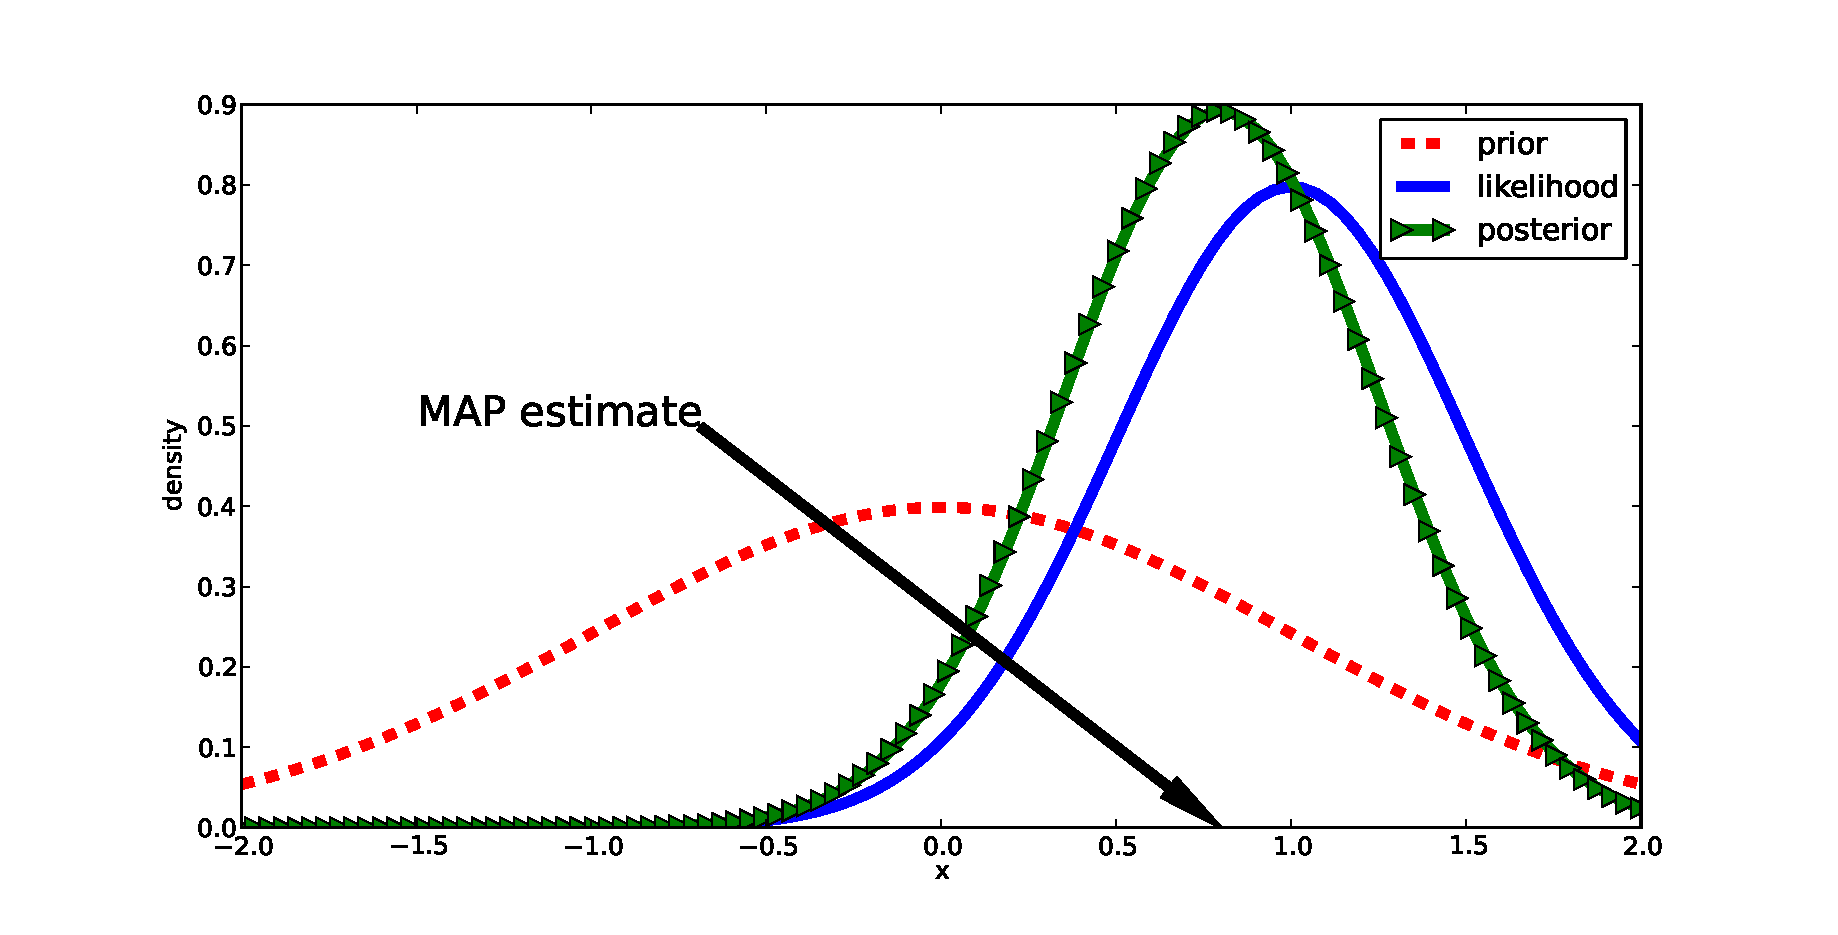
\includegraphics[width=\textwidth]{../images/gaussian-bayesian}
  \caption{The posterior is a compromise between the prior and the likelihood.}
  \label{linear:fig:gaussian-bayesian}
\end{figure}
Since the term involving $\|w\|^2$ is a sum of $K$ components, and the term involving $Y_1$ is a scalar equation, the $\|w\|^2$ term will dominate the posterior unless $w$ is small.  Therefore,  the $w$ that maximizes the posterior, $w_{map}$ will be small.  In other words, our best guess will look like a likely draw from the prior.  In this way, the posterior is a compromise between the prior and likelihood (see figure \ref{linear:fig:gaussian-bayesian}).  Specifically:
\begin{itemize}
  \item If our noise variance $\sigma_\eps^2$ was huge, then our posterior would be dominated by the prior, and our best guess $w_{map}$ would be close to zero. 
  \item If \emph{a priori} we were certain that $w_{true}$ was close to zero, then $\sigma_w$ would be small.  As a result, the $\|w\|^2$ term would be highly dominant and $w_{map}\approx0$.
  \item The likelihood slightly perturbs $w_{map}$ in a direction that fits the data.
  \item It is easy to show that the right hand side of the above minimization problem is strictly convex, so one unique solution exists.
\end{itemize}

Once we include all $N$ experiments, our posterior is
\begin{align*}
  p(w\g Y) &\propto p(Y\g w)p(w) \\
  & = p_E(Y-Xw)p(w) \\ 
  & = \exp\left\{ -\frac{1}{2\sigma_\eps^2}\|Xw-Y\|^2 \right\}\exp\left\{-\frac{1}{2\sigma_w^2}\|w\|^2\right\}.
\end{align*}
Since the product of two Gaussians is Gaussian, our posterior is Gaussian.  Our MAP solution becomes
\begin{align}
  w_{map} :&= \arg\min_w \left[  \frac{\|Xw-Y\|^2}{\sigma_\eps^2} + \frac{\|w\|^2}{\sigma_w^2}\right].
  \label{linear:align:gaussian-map}
\end{align}
Now the term $\|Xw-Y\|^2 = \sum_{n=1}^N|X_{n:}\cdot w - Y_n|^2$ is a sum of $N$ terms.  If $N\gg K$ (if we have much more data than unknowns), it will dominate and $w_{map}$ will be chosen to fit the data.

\begin{exercise}
  \label{linear:exercise:overfitting-simple}
  Show that adding more covariates to $w$ can only decrease $\|X w-Y\|$.  Does this mean that adding more covariates is always a good idea?
\end{exercise}

\begin{exercise}
  Derive \eqref{linear:align:gaussian-map}.
\end{exercise}

\begin{exercise}
  What happens to the MAP estimate as your prior uncertainty about $w$ goes to infinity (e.g. $\sigma_w\to\infty$)?  Does this seem reasonable?
\end{exercise}


The omnipotent house cat was introduced to emphasize the fact that this ideal world does not exist.  In real life, our unmodeled response $E_n$ depends on $X_{n:}$ and is certainly not Gaussian.  Furthermore, what does $w$ represent in real life?  Suppose we take the interpretation that $w$ is a vector of derivatives of the input/output response, then for what reason would our prior guess be $w\sim\calN(0, \sigma^2_wI_K)$?  All however is not lost.  If your model is not too far from reality, then your interpretation of $w$ will have meaning, and your predictions will be accurate.  This is what mathematical modeling is.  The beauty of the Bayesian approach is that it makes these assumptions explicit.  In the next section, we will see how our inevitable misspecification of error along with data quality issues will degrade our estimation/prediction, and the prior will take on the role of preventing this degradation from getting out of hand.

\section{Coefficient Estimation: Optimization Formulation}
\label{linear:section:optimization}
As we saw in section \ref{linear:section:bayesian}, in the case of Gaussian prior and error, finding the ``best guess'' coefficient $w_{map}$, is equivalent to solving the \emph{regularized least squares} optimization problem:
\begin{align}
  w_{map} :&= \arg\min_w \left\{ \|X w - Y\|^2 + \delta\|w\|^2 \right\},
  \label{linear:align:optimization}
\end{align}
with $\delta = \sigma^2_\eps/\sigma^2_w$.
In addition, solving the maximum likelihood problem gives us the classic least squares problem of finding a $w$ such that $X w$ best approximates $Y$.
\begin{align}
  w_{lq} :&= \arg\min_w \quad \|X w - Y\|^2.
  \label{linear:align:lsq}
\end{align}

% TODO Move to after remark 6.11 (after the lsq problem is solved by SVD)
\begin{exercise}
  Suppose $X\in\RNK$ and $Y\in\RN$.  In other words, suppose you take $N$ measurements and use $K$ covariates (possibly including a constant).  
  \begin{enumerate}
    \item What are the conditions on $N$ and $K$ and the rank of $X$ that ensure we have a unique solution to the unregularized least squares problem?
    \item What are the conditions on $N$ and $K$ and the rank of $X$ that ensure we have an infinite number of solutions to the unregularized least squares problem?
    \item What are the conditions on $N$ and $K$ that prevent us from having any solution to $X w=Y$ for every $Y$?
  \end{enumerate}
\end{exercise}

Solving the least squares problem can be done explicitly by multiplying both sides by $X^T$, yielding the \emph{normal equations}
\begin{align*}
  X^TXw_{ls} &= X^TY. 
\end{align*}
Assuming $X^TX$ is nonsingular, we can (in principle) invert it to find $w_{ls}$ (note that at this point we have not proved this actually finds the $w$ that minimizes \eqref{linear:align:lsq}).
\begin{align*}
  w_{ls} &= (X^TX)^{-1}X^TY,\qquad \mbox{ assuming $X^TX$ is non-singular}.
\end{align*}
Plugging $Y = Xw_{true} + E$ into this we have
\begin{align*}
  w_{ls} &= (X^TX)^{-1}X^TXw_{true} + (X^TX)^{-1}X^TE\\
  &= w_{true} + (X^TX)^{-1}X^TE ,\qquad \mbox{ assuming $X^TX$ is non-singular}.
\end{align*}
The second term is error that we hope is small.  Roughly speaking, if $X$ ``squashes'' some signals, then $(X^TX)^{-1}$ will make some noise terms ``blow up.''  The balance between how our variable selection picks out signals and how our inversion blows up noise is a delicate interplay of a special basis that we will study in the next section.


\subsection{The least squares problem and the singular value decomposition}
Here we study the singular value decomposition.  This decomposition is useful for analyzing and solving the least squares problem \eqref{linear:align:optimization}.  It is also the basis of methods such as Principle Component Analysis (PCA).  To motivate the SVD consider the lucky 
situation where your covariate matrix was diagonal, e.g.
\begin{align*}
  X &= \left( 
  \begin{matrix}
  2 & 0\\
  0 & 3
  \end{matrix}
  \right)
\end{align*}
We then have 
\begin{align*}
  Xw &= Y \Leftrightarrow \left( 
  \begin{matrix}
    2w_1\\3w_2
  \end{matrix}
  \right) = \left( 
  \begin{matrix}
    Y_1 \\ Y_2
  \end{matrix}
  \right),
\end{align*}
from which it easily follows that $w_1 = Y_1/2$, and $w_2 = Y_2/3$.  If $X$ were not diagonal but were symmetric, we could find a basis of eigenvectors $(v_1, v_2)$ such that $Xv_k = \lambda_kv_k$.  We then write $Y = (Y\cdot v_1)v_1 + (Y\cdot v_2)v_2$, and $w = \tilde w_1v_1 + \tilde w_2v_2$.  We then have $Xw=Y$ if and only if
\begin{align*}
  \lambda_1\tilde w_1v_1 + \lambda_2\tilde w_2 v_2 &= (Y\cdot v_1)v_1 + (Y\cdot v_2)v_2,
\end{align*}
which implies $\tilde w_1 = (Y\cdot v_1)/\lambda_1$ and $\tilde w_2 = (Y\cdot v_2)/\lambda_2$.  
\begin{example}
  \label{linear:example:eigendecomp}
  Consider the matrix 
  \begin{align*}
    X = \left( 
    \begin{matrix}
      2 & 1\\
      1 & 2
    \end{matrix}
    \right).
  \end{align*}
  \begin{itemize}
    \item Show that $v_1 = 2^{-1/2}(1,1)$ and $2^{-1/2}(-1,1)$ are an orthonormal basis for $\Rtwo$
    \item Show that $v_1$ and $v_2$ are eigenvectors of $X$
    \item Use that fact to find $w$ such that $Xw = (3, 4)$.
  \end{itemize}
\end{example}

An eigenvalue decomposition such as in example \ref{linear:example:eigendecomp} is possible for $X$ only if $X^TX=XX^T$.  This is never the case for non-square matrices.  Fortunately a singular value decomposition is always possible.

\begin{definition}[Singular Value Decomposition (SVD)]
  \label{linear:definition:svd}
A singular value decomposition of a matrix $X$ is a set of \emph{left singular vectors} $\left\{ u_1,\cdots,u_N \right\}$, a set of \emph{right singular vectors} $\left\{ v_1,\cdots,v_K \right\}$, and a set of \emph{singular values} $\left\{ \lambda^2_1,\cdots,\lambda^2_{N\vee K} \right\}$ ($N\vee K$ is the maximum of $N$ and $K$) such that
\begin{itemize}
  \item The $v_k$ form an orthonormal basis for $\RK$
  \item The $u_n$ form an orthonormal basis for $\RN$
  \item $Xv_j = \lambda_ju_j$, and $X^Tu_j=\lambda_jv_j$ for $j=1,\cdots,N\vee K$
  \item $\lambda_1\geq\lambda_2\geq\cdots\geq\lambda_{N\vee K}\geq0$, and if $K\leq N$, we have an $r\leq K$ such that $\lambda_{r+1}=\cdots=\lambda_N=0$.
\end{itemize}
\end{definition}
This decomposition is also sometimes written 
\begin{align}
  X &= U\Sigma V^T,
  \label{linear:align:svd}
\end{align}
where the columns of $U$ are the $u_j$, the columns of $V$ are the $v_j$, and $\Sigma\in\RNK$ has the $\lambda_j$ on its diagonal (as far as its diagonal actually goes since it is not necessarily square\ldots). 

\begin{exercise}
  Show that \eqref{linear:align:svd} follows from definition \ref{linear:definition:svd}.
\end{exercise}

\begin{exercise}
  Show that the right singular vectors (the $v_j$) are the eigenvectors of the matrix $X^TX$, and the singular values are the square roots of the eigenvalues.
  \label{linear:exercise:svd-eigen}
\end{exercise}

\begin{digression}[Simplifying Basis]
  The SVD of $X$ is a choice of basis under which the operator $X$ acts in a simple manner:  $Xv_k=\lambda_ku_k$.  This ``trick'' is widely used in mathematics.  The most famous example is probably the Fourier series.  Here, one chooses a sinusoidal basis to transform functions:
  \begin{align*}
    f(x) &= \sum_{k=1}^\infty f_k\sin2\pi kx.
  \end{align*}
  The differential operator $\d^2/\dx^2$ then takes the simple action
  \begin{align*}
    \frac{\d^2}{\dx^2}\sin2\pi kx &= -(\pi k)^2\sin2\pi kx.
  \end{align*}
  This is useful algebraically but also intuitively because nature tends to treat low and high frequencies differently (low frequency sounds travel further in water for example).  The same is true of all \emph{compact} operators (matrices being one example of this).  For that reason, we often refer to the ``tail end'' of the singular values (e.g. $\left\{ v_{N-3}, v_{N-2}, v_{N-1}, v_N \right\}$) as higher frequencies.
\end{digression}

Assuming one has an SVD of $X$ (computing that will be saved for later), we can solve the unregularized least squares problem.  Start by using the fact that the $u_n$ form an orthonormal basis to write
\begin{align*}
  Y &= \sum_{n=1}^N (u_n\cdot Y)u_n.
\end{align*}
We now seek to find a solution $w$ of the form 
\begin{align*}
  w &= \sum_{k=1}^K \tilde w_k v_k.
\end{align*}
The coefficients are written $\tilde w_k$ to emphasize that these are not the coefficients in the standard Euclidean basis.  For simplicity, let's assume a common case that $K\leq N$ and inserting the expressions for $Y$ and $w$ into $\|Xw-Y\|^2$.  This yields
\begin{align*}
  \left\|Xw - Y\right\|^2 &= \left\| X\sum_{k=1}^K\tilde w_k v_k - \sum_{n=1}^N(u_n\cdot Y)u_n\right\|^2 \\
    &\quad= \left\| \sum_{k=1}^K\tilde w_k\lambda_k u_k - \sum_{n=1}^N(u_n\cdot Y)u_n\right\|^2 \\
    &\quad= \left\| \sum_{k=1}^r(\tilde w_k\lambda_k - (u_k\cdot Y))u_k - \sum_{n=r+1}^N(u_n\cdot Y)u_n\right\|^2 \\
    &\quad= \sum_{k=1}^r \left( \tilde w_k\lambda_k - (u_k\cdot Y) \right)^2 + \sum_{n=r+1}^N(u_n\cdot Y)^2.
\end{align*}
The fourth equality follows since the $u_n$ are orthonormal.  
\begin{remark}
  \label{linear:remark:svd-soln}
We note a few things:
\begin{itemize}
  \item If $N>K$, there is an exact solution to $Xw=Y$ if and only if $u_n\cdot Y=0$ for $n>r$.
  \item Solutions to the unregularized least squares problem \eqref{linear:align:lsq} are given by:
    \begin{align*}
      \tilde w_k &= \left\{ 
        \begin{matrix}
          &(u_k\cdot Y)/\lambda_k,\quad 1\leq k\leq r\\
          &\mbox{anything},\quad r+1\leq k\leq K.
        \end{matrix}
      \right\}
    \end{align*}
  \item Setting $\tilde w_k\equiv0$ for $k>r$ gives us the so-called \emph{minimal norm solution}.
    \begin{align*}
      \arg\min\left\{ \|\hat w\|^2\st \hat w \mbox{ is a solution to \eqref{linear:align:lsq}}\right\}.
    \end{align*}
  \item The (Moore-Penrose) \emph{pseudoinverse} $X^\dagger$ is defined by
    \begin{align*}
      X^\dagger Y &= \sum_{k=1}^r \frac{u_k\cdot Y}{\lambda_k}v_k.
    \end{align*}
    In other words, $X^\dagger Y$ is the minimal norm solution to the least squares problem.  One could just as easily truncate this sum at $m\leq r$, giving rise to $X^{\dagger,m}$.
\end{itemize}
\end{remark}

There exist a variety of numerical solvers for this problem.  So long as the number of covariates $K$ is small, most will converge on (approximately) the solution given above.  The $1/\lambda_k$ factor however can cause a huge problem as we will now explain.  Recall that our original model was:
\begin{align*}
  Y &= Xw_{true} + E = \sum_{k=1}^K (w_{true}\cdot v_k)\lambda_k u_k + \sum_{n=1}^N(E\cdot u_n)u_n.
\end{align*}
Inserting this into the expression $\tilde w_j = (u_j\cdot Y)/\lambda_j$, we have
\begin{align}
  \begin{split}
    \tilde w_j &= w_{true}\cdot v_j + \frac{E\cdot u_j}{\lambda_j}
    = \frac{\lambda_j(w_{true}\cdot v_j) + E\cdot u_j}{\lambda_j}
    = \frac{\left[ Xw_{true} + E \right]\cdot u_j}{\lambda_j}.
  \end{split}
  \label{linear:align:coefficient-with-error}
\end{align}

The term $Xw_{true}\cdot u_j$ is our modeled output in direction $u_j$.  Similarly, $E\cdot u_j$ is a measure of the unmodeled output in direction $u_j$.  If our unmodeled output in this direction is significant, our modeling coefficient $\tilde w_j$ will differ from the ``true'' value.  Moreover, as $\|Xv_j\| = \|\lambda_ju_j\| = \lambda_j$, the singular value $\lambda_j$ can be seen as the magnitude of our covariates pointing in direction $v_j$.  If our covariates did not have significant power in this direction, the error in $\tilde w_j$ will be amplified.  Thus, the goal for statistical inference of coefficients is clear:  Either avoid this ``large error'' scenario (by modeling better and avoiding directions in which your data is sparse) or give up on modeling these particular coefficients accurately.  For prediction the situation isn't so clear.  Suppose we have a new input $x$.  Our ``best guess'' output is 
\begin{align}
  \begin{split}
    \hat y = x\cdot \tilde w & = \left( \sum_{k=1}^K(x\cdot v_k)v_k \right)\cdot \left( \sum_{k=1}^K \left[ \frac{\left[ Xw_{true} + E \right]\cdot u_k}{\lambda_k} \right]v_k\right) \\
    &= \sum_{k=1}^K(x\cdot v_k)\left[ \frac{ \left[ Xw_{true} + E \right]\cdot u_k}{\lambda_k} \right].
  \end{split}
  \label{linear:align:fundamental}
\end{align}
Assume we are in the ``large error'' scenario as above.  Then the term in square brackets will be large.  If however the new input $x$ is similar to our old input, then $x\cdot v_j$ will be small (on the order of $\lambda_j$) and the error in the $j^{th}$ term of our prediction will be small.  In other words, if your future input looks like your training input, you will be ok.

\begin{exercise}
  Assume we measure data but one variable is always exactly the same as the other.  What does this imply about the rank of the variable matrix $X$?  Show that this means we will have at least one singular value $\lambda_k=0$ for $k\leq K$.  Since singular values change continuously with matrix coefficients, this means that if two columns are almost the same then we will have a singular value $\lambda_k\ll1$.  This is actually more dangerous since if $\lambda_k=0$ your solver will either raise an exception or not invert in that direction, but if $\lambda_k\ll1$ most solvers will go ahead and find a (noisy) solution.
\end{exercise}

\begin{exercise}
  Using \eqref{linear:align:coefficient-with-error} show that if $X$ and $E$ are independent, then $\Exp{w} = w_{true}$.

  Note that since $\lambda_j\sim O(N)$ and in the uncorrelated case $E\cdot u_j\sim O(\sqrt{N})$, one can show that if the errors are uncorrelated with the covariates then $w\to w_{true}$ as $N\to\infty$.
\end{exercise}

\subsection{Overfitting examples}
The next exercise and example are instances of \emph{overfitting}.  Overfitting is a general term describing the situation when the noise term in our training data $E$ has too big an influence on our model's fit.  In this case, our model will often fit our training data well, but will not perform well on future data.  The reason is that we have little understanding of the noise term $E$ and very little understanding of what it will do in the future.  

\begin{example}
The most classic example is that of polynomial fitting.  Suppose our actual data is generated by
\begin{align}
  y = x + x^2 + x^3 + \eps(x), \quad x=0, 0.1,\cdots,1.0.
  \label{linear:align:poly}
\end{align}
We fit this data by minimizing the mean square error of both three and six degree polynomials (equivalently maximizing the obvious likelihood function).  This can be done with the following Python code.

\rule{\textwidth}{2pt}
\begin{minted}{python}
import scipy as sp
import matplotlib.pyplot as plt 

x = sp.linspace(0, 1, 10) 
x_long = sp.linspace(-0.1, 1.1, 100)

y = x + x**2 - x**3 + 0.1 * sp.randn(len(x))

z = sp.polyfit(x, y, 3)
p = sp.poly1d(z)
print "3-degree coefficients = %s" % z 

z6 = sp.polyfit(x, y, 6)
p6 = sp.poly1d(z6)
print "6-degree coefficients = %s" % z6

plt.clf()
plt.plot(x, y, 'b.', ms=18, label='Y')
plt.plot(x_long, p(x_long), 'r-', lw=5, label='3-degree poly')
plt.plot(x_long, p6(x_long), 'g--', lw=6, label='6-degree poly')
plt.xlabel('X')
plt.legend(loc='best')

plt.show()
\end{minted}
\rule{\textwidth}{2pt}

See figure \ref{linear:figure:polyfit}.
\begin{figure}
  \label{linear:figure:polyfit}
  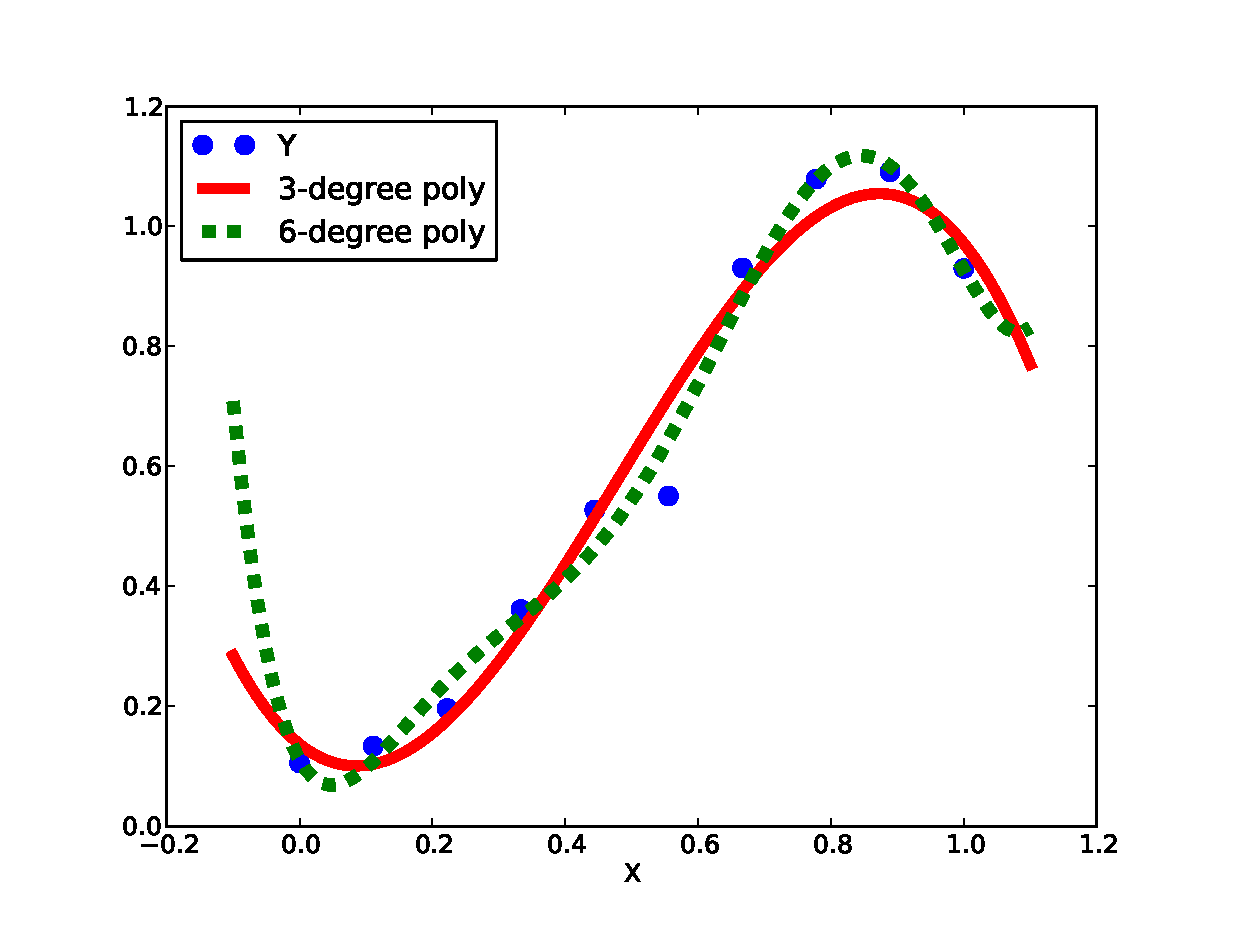
\includegraphics[width=0.7\textwidth]{../images/polynomial}
  \caption{Polynomial fitting and overfitting}
\end{figure}
The third degree polynomial fits well but not perfectly at every point.  The six degree polynomial fits the data better, but wiggles in a ``crazy'' manner, and looks like it will ``blow up'' outside the range of $[0,1]$.  Furthermore, running this code multiple times shows that all coefficients in the six degree polynomial are highly dependent on the error and the first three terms are no where near the real terms.  For statistical inference this is a killer:  How can you report these coefficients as ``findings'' when they so obviously depend on the unmodeled noise?  For prediction the situation is slightly more nuanced.  If we believe future $x$ values will fall outside the interval $[0,1]$, then we are clearly in trouble.  On the other hand, if future values lie inside this interval then it can be seen that our polynomial, no matter how crazy it is, will predict quite well.  Beware however:  In higher dimensions it becomes difficult to determine the range of applicability of your model.  It is usually better to be safe and error on the side of underfitting.  Note that this is an example of the more general result of equation \eqref{linear:align:fundamental}.
\end{example}


\begin{exercise}[Misspecification of error correlations]
  Let's model percentage stock returns among four different stocks (the relative percentage change in stock price over one day).  We will model the tomorrows returns as depending on todays returns via the relation $y = w_1x + w_2x^2 + \eps$, where $\eps$ is uncorrelated for every stock (recall that ordinary least squares implicitly makes this assumption).  Let's assume the real life model is $y = x + 0.05x^2 + \eta$, where $\eta$ for different stocks is sometimes uncorrelated and sometimes correlated. Since, on most days, returns are around $\pm1\%$, we have approximately a 10 to 1 signal to noise ratio and think that we're ok.  Taking measurements of the stock prices on one day we get our data matrix (first column is the returns, second column is the squared returns).
  \begin{align}
    X &= \left( 
    \begin{matrix}
      1 & 1\\
      -1 & 1 \\
      1 & 1 \\
      -1 & 1
    \end{matrix}
    \right).
    \label{linear:align:bad-matrix}
  \end{align}
  \begin{enumerate}
    \item Use exercise \ref{linear:exercise:svd-eigen} to show that the right singular vectors are $v_1=(1,0)^T$, and $v_2=(0,1)^T$, and the singular values are $\lambda_1=\lambda_2=2$.
    \item Use the fact that $Xv_j = \lambda_ju_j$ to show that $u_1=0.5\cdot(1, -1, 1, -1)^T$, and $u_2=0.5\cdot(1, 1, 1, 1)^T$.
    \item Suppose we measured returns the day after and got $Y = (1.25, -1.15, 0.85, -0.75)^T$.  One could use $y = x + 0.05x^2 + \eta$ to explicitly calculate $\eta$ and infer that the noise was basically uncorrelated (all 4 $\eta$ were not related).  Use remark \ref{linear:remark:svd-soln} to show that our estimate for $w$ is $(1, 0.05)$, which is the exact result in the uncorrelated model.  Note:  Since $(v_1, v_2)$ are the standard basis, the coefficients for $w$ estimated by \ref{linear:remark:svd-soln} will be in the standard basis as well.
\item Suppose instead that we measured $\tilde Y=(1.15, -0.85, 1.15, -0.85)$.  So the noise was correlated.  Show that our estimate is $w = (1, 0.15)$.  The coefficient for $w_2$ was three times larger than before!
\item What will happen if we use the second coefficient to predict returns during uncorrelated times?  What about during times when the error is negative and correlated?   What about positive and correlated?
  \end{enumerate}
  Note that if errors were always correlated, say with correlation matrix $\Sigma$, one should solve the generalized least squares problem:
  \begin{align*}
    \hat w &= \arg\min_w (Xw - Y)^T\Sigma^{-1}(Xw-Y).
  \end{align*}
  This can be seen by reworking the example in section \ref{linear:subsection:gaussian-example}, starting with the assumption $E\sim\calN(0, \Sigma)$.

  One could also take the viewpoint that while we cannot hope to specify the error model correctly, we do know \emph{a priori} that the coefficient of $x^2$ should be smaller than that of $x$.  In this case, we could use a prior proportional to 
  \begin{align*}
    \exp\left\{ -\frac{1}{2}\left[ \frac{w_1^2}{2\lambda_w^2} + \frac{w_2^2}{2\cdot0.1\cdot\lambda_w^2} \right] \right\}.
  \end{align*}
  Alternatively, we could fit our model to fake data that was perturbed by different noise models.  If the results show wild swings in the coefficients then we should be cautious.
\end{exercise}

\begin{example}
  \label{linear:example:small-singular-values}
Another example starts with the data matrix
\begin{align*}
  X &= 
  \left( 
  \begin{matrix}
    1 & 1.01\\
    1 & 1
  \end{matrix}
  \right).
\end{align*}
This matrix is almost singular because the two rows are almost the same.  This happened because, over our measured data set, the two covariates were almost the same.  If our model is good, we expect the two measured responses $Y_1$, $Y_2$ to be almost the same (either that or we have some pathological case such as $y = 1000(x_1 - x_2)$).  One finds that the singular values are $\lambda_1=2.005$, $\lambda_2=0.005$.  The smaller singular value is a problem.  It is associated with the singular directions $v_2=(0.71, -0.71)$, $u_2=(-0.71, 0.71)$.  This means that 
\begin{align*}
  0.71(w_1 -w_2) = \tilde w_2 &= 200\cdot0.71(Y_2 - Y_1).
\end{align*}
In other words, our coefficient is extremely sensitive to $Y_1-Y_2$.  Small differences between the two will lead to a huge difference in $w$ (note that this will not lead to huge changes in $w_1+w_2$, only $w_1-w_2)$.  The upshot is that our predictive model will work fine so long as future $x$ values have $x_1\approx x_2$ (just like our training data), but if we stray outside the range of our training data we are in for big problems.
\end{example}

\subsection{$L_2$ regularization}
As was mentioned earlier, the Bayesian MAP problem reduces, in the Gaussian case, to the optimization problem
\begin{align}
  w_\delta :&= \arg\min_w \left\{ \|Xw - Y\|^2 + \delta\|w\|^2 \right\}.
  \label{linear:align:regularized-lsq}
\end{align}
With ``no math'' whatsoever, one can see that the \emph{penalty term} $\|w\|^2$ acts to prevent $w$ from becoming too big.  As with classical least squares, the SVD provides insight into exactly what is happening.

\begin{theorem}
  If $\delta>0$ then the solution to \eqref{linear:align:regularized-lsq} exists, is unique, and is given by the formula
  \begin{align*}
    w_\delta &= (X^TX + \delta I)^{-1} X^TY = \sum_{k=1}^K \frac{\lambda_k}{\lambda_k^2 + \delta}(Y\cdot u_k)v_k
  \end{align*}
  \label{linear:theorem:regularized-lsq}
\end{theorem}
\begin{proof}
  The second equality follows from definition \ref{linear:definition:svd} and exercise \ref{linear:exercise:svd-eigen}.  To show the first equality let $F(w):= \|X w-Y\|^2 = \delta\|w\|^2$.  We then have, for any vector $z$,
  \begin{align*}
    F(w_\delta+z) &= F(w_\delta) + 2z^T\left( (X^TX + \delta I)w_\delta - X^TY \right) + \|X z\|^2 + \delta\|z\|^2 \\
    &= F(w_\delta) + \|X z\|^2 + \delta\|z\|^2.
  \end{align*}
  Since the second term vanishes only when $z=0$, we see that $F(w_\delta+z)$ is minimized when $z=0$.  Thus $w_\delta$ minimizes $F$ and we are done.
\end{proof}

\begin{remark}
  As $\delta\to0$ it is easy to see that the regularized solution converges to the minimal norm solution.  For $\delta>0$ the solution components associated with the smaller singular values are attenuated more.  This is fortunate since these components can be quite troublesome as example \ref{linear:example:small-singular-values} has shown.  
\end{remark}

\subsection{Choosing the regularization parameter}
\label{linear:subsection:cross-validation}
Much has been written on techniques (Bayesian or otherwise) to choose optimal regularization parameters.  These (asymptotic) optimality results usually rely on assumptions about the error model (i.e. that your error model is correct or ever that the error is uncorrelated to the covariates).  This is unfortunate since this is usually not the case.  There is also the method of \emph{hierarchical Bayesian} modeling.  Here, the prior is left unspecified and the data determines it.  While accepting that these results do have their place we prefer instead to show the simple method of \emph{cross validation}.  

A typical cross validation cycle would go as follows:
\begin{enumerate}
  \item Choose a number of possible values for $\delta$, call them $(\delta_1,\cdots,\delta_M)$.  For every $\delta_m$\ldots
  \item Segregate your observations into a \emph{training set} $X^{train}$, $Y^{train}$ and a \emph{cross validation set} $X^{cv}$, $Y^{cv}$.  A common split would be 70-30.
  \item For every $\delta_m$, use the training data to solve the regularized least squares problem \eqref{linear:align:regularized-lsq} obtaining $(w_{\delta_1},\cdots,w_{\delta_M})$.
  \item For every $m$, measure the \emph{cross validation error} (here it is a relative root-mean-square error) $\|X^{cv}w_{\delta_m} - Y^{cv}\|/\|Y^{cv}\|$.
  \item Choose $\delta$ to be the $\delta_m$ that minimizes that error.
  \item Train your model using the full data set and $\delta$ from above.
\end{enumerate}

Step 1 chooses a bigger set of data for training than cross validation.  This is typical because you are training $K$ different parameters, but (in this case) only using cross validation to find one.  Thus, we are not worried so much about overfitting a small data set.  The $\delta_m$ in step 2 are usually picked by first guessing a few values of $\delta$ and seeing over what range of values the training data misfit isn't too horrible.  In step 3 we solve the regularized problem multiple times.  Note that if we were to measure the training data (unregularized) least squares error $\|X^{train}w_{\delta_m}- Y^{train}\|/\|Y^{train}\|$ we would see the training error get worse monotonically as $\delta$ increases.  What we care about (and measure in step 4) is the cross validation set error.  The hope is that the error $\eps^{cr}$ will be such that problems associated with overfitting show up here.  Note that there is nothing canonical about the choice of error in step 4.  If for example you care more about large errors, a fourth order error function could be used.  In step 5 we choose $\delta$ as the minimizer of the cross validation error.  Again, different choices could be made.  For example, one may have generated the training and cross validation sets by sampling people in 2010.  It may or may not be reasonable to believe people in 2013 will act according to the same model.  If they don't the error function $\eps(x,z)$ could be much different and this could cause your model to behave poorly when fed with 2013 data.

\begin{exercise}
  Use the SVD to show that the mean square training error gets worse monotonically with increasing $\delta$.
\end{exercise}

Unlike the training (mean square) error, the cross validation error does not always change monotonically.  If for example, the variable matrix $X$ had highly correlated columns, then the singular values will rapidly decrease.  This in turn causes an overfitting effect.  In our idealized $Y = Xw + E$ world this means that $\hat w$ will be far from $w_{true}$.  As a result, the cross validation error will (on average) be convex (see figure \ref{linear:fig:overfitting} left).  If on the other hand your variables were uncorrelated, then there is no reason to believe that the model will overfit to the noise, and it is possible that both training and cross validation error will monotonically increase (see figure \ref{linear:fig:overfitting} right).  The reader is cautioned however that in the ``real world'' the data is not generated by $Y = Xw + E$ with uncorrelated $E$, and more complex behaviors can emerge.  In particular, the modeler may intend on using the model on real-world inputs that behave differently than the training (or cross-validation) input.  For example, both the training and cross validation data could be from pre 2008 (before the financial crisis) but you will use your model in a post 2012 world.  These \emph{out of time} errors can be especially problematic.  In this case, the modeler can error on the side of caution and use more regularization than the cross-validation cycle above suggests.  Another popular method is to reduce the number of variables to a smaller set that is human interpretable (e.g., a human can check that the coefficient in front of a particular variable is reasonable).

\begin{figure}
  \label{linear:fig:overfitting}
  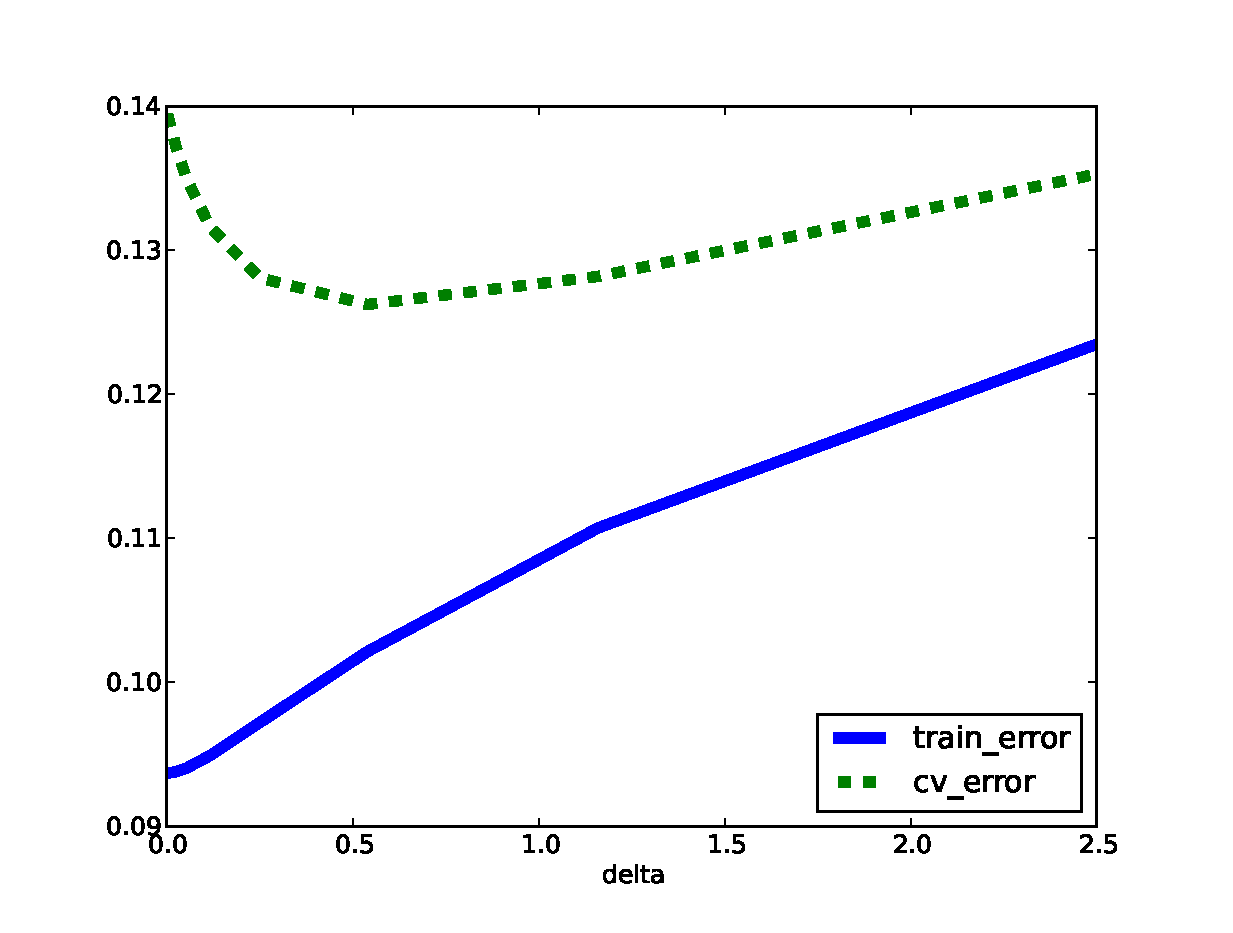
\includegraphics[width=0.5\textwidth]{../images/train-cv-error}
  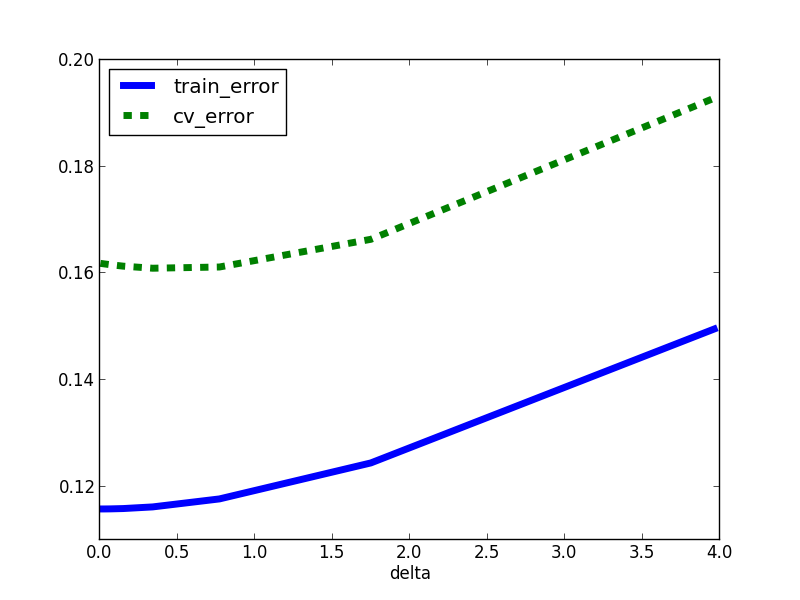
\includegraphics[width=0.5\textwidth]{../images/train-cv-error2}
  \caption{Cross validation and test errors.  Left:  The $X$ matrix with correlated columns, hence the unregularized solution was overfitting.  Right:  The $X$ matrix had uncorrelated columns and therefore the unregularized solution was not overfitting.}
\end{figure}

\subsection{Numerical techniques}
\label{linear:subsection:numerical}
The conclusion of theorem \ref{linear:theorem:regularized-lsq} implies that one can find $w_\delta$ by solving:
\begin{align}
  (X^TX + \delta I)w_\delta &= X^TY.
  \label{linear:align:reg-problem}
\end{align}
It is easy to show that the condition number of $A:=(X^TX + \delta I)$ is at least as large as $\delta$.  So when $\delta>0$ is large enough the problem is well-posed and can be solved directly even for large $N, K$ (e.g. $N=K=1000$ gives little trouble).  If $\delta=0$ and columns of $X$ are linearly dependent, you will not be able to invert $X^TX$.   Even if $X^TX$ is invertible in theory, if $\delta$ is small then numerical error can cause error (e.g. when the condition number is in the millions).

Alternatively, one can compute the SVD of $X$ and then use the pseudoinverse $X^\dagger$.  This has the advantage of not having to worry about linearly dependent columns (sometimes however is is often nice to know that your columns are dependent).  Moreover, computing the SVD of $X$ can be done in a stable manner even for large matrices.

The ``best'' alternative for small or medium matrices is to factor the matrix into a simpler form.  One example is the $QR$ factorization.  We write $X^TX = QR$ with $Q$ orthogonal and $R$ upper triangular.  The resultant normal equations ($QRw = X^TY$) are then trivial to solve.  First we multiply by $Q^T$ (which is $Q^{-1}$), then solve the system of equations $Rw = Q^TX^TY$ (which is trivial since $R$ is triangular).  This has the advantage of being numerically very stable and quicker than the SVD.  

The methods described so far are not suited for larger problems because they require the full matrix to exist in memory, and attempt to completely solve the problem (which is difficult and unnecessary for large problems).  In this case, an iterative technique is used.  Here we start with a guess $w^0$, and iteratively improve it until we have reduced the \emph{residual} $\|Xw^\ell - Y\|$ to a small enough value.  These iterative techniques typically require evaluation of $Xu$ for various vectors $u$.  This does not require storing $X$ (you only need to stream $X$ in and out of memory, and multiply things while things are in memory).  For the case of a large sparse (most entries are zero) you can store the nonzero values and use these to perform multiplication.  Moreover, rather than completely solving the problem, you can stop at any point and obtain an approximate solution.


\section{Variable Scaling and Transformations}
To motivate this section, consider the linear model $y = w_1 + w_2x +\eps$, where $y$ is ``wealth'', and $x$ is a person's height.  If height is measured in millimeters, then $x$ will be around 1,500.  If on the other hand height is measured in meters, then $x$ will be around 1.5.  Intuition tells us that when height is measured in millimeters (and thus $x$ is very large), the optimal $w_1$ will be much smaller.  This is a form of prior belief.  This section will conclude:
\begin{enumerate}
  \item Maximum likelihood estimation require no special attention to variable scale (except for possible numerical issues) to produce optimal coefficients.
  \item Bayesian estimates will be flawed unless the prior is adjusted in accordance with variable scale (or the variables all have the same scale).
  \item In all cases, scaled variables are often easier to interpret.
\end{enumerate}
\subsection{Simple variable scaling}
Returning to our height example, suppose we use millimeters and find an optimum $w_{ml}$ using least squares.  In other words, 
\begin{align*}
  w_{ml} &= \arg\min_w \sum_{n=1}^N \left( w_0 + w_1 X_{n1} - Y_n \right)^2.
\end{align*}
Suppose we change to meters.  Then the heights, $X_{n1}$, change to $\tilde X_{n1} = X_{n1}/1000$.  We then seek to find $\tilde w_{ml}$, the maximum likelihood solution in these new variables.  Rather than re-solving the problem, we can write the above equation as
\begin{align*}
  w_{ml} &= \arg\min_w \sum_{n=1}^N \left( w_0 + w_1\cdot1000 \cdot\frac{X_{n1}}{1000} - Y_n \right)^2 \\
  &= \arg\min_w \sum_{n=1}^N \left( w_0 + w_1\cdot1000 \cdot\tilde X_{n1} - Y_n \right)^2.
\end{align*}
Since $w_{ml}= ( (w_{ml})_0, (w_{ml})_1)$ minimizes the above sum, we see that the minimizing multiplier of heights (in meters) is $w_1\cdot1000$.  Therefore, $\tilde w_{ml} = ( (w_{ml})_0, 1000\cdot(w_{ml})_1)$.  In other words, when the variable $x$ got 1000 times smaller, its coefficient got 1000 times larger.  In either case, solving a simple least squares problem should produce the correct answer.  In both cases, the residual error $\|Xw_{ml}-Y\|^2$ will be the same. 

Although we are in theory able to ignore variable scaling, practical matters make us reconsider.  Recalling our discussion in previous sections, we would like to use huge variables as an common symptom of overfitting. Note however that in one case the second component of $w_{ml}$ is 1000 times larger than the other case.  So we obviously cannot look at raw coefficient magnitude as a symptom of overfitting.  Moreover, the normal matrix $X^TX$ will have bottom right entry equal to $\sum_n X_{n1}^2$, which could be huge if we are using millimeters.  Many linear algebra packages would have trouble solving maximum likelihood problem.  In other cases this sum could be so large or small that our computer cannot store it.  Suppose further that we used both \emph{height} and \emph{health} as variables.  Then, our choice of units to represent height/health in would influence the absolute values of our coefficients.  We would not be able to say, ``the coefficient of height is 10 times larger, and therefore height is probably more important.''  Although this is not the proper way to conclusively judge variable importance, it is a good way to get rough guesses that can be used to find model issues (e.g. if the coefficient of health was almost zero, we should be surprised).

The most common solution to this issue is to rescale columns of $X$ by the sample standard deviation of the columns.  In other words, with 
\begin{align*}
  \mu_k :&= \frac{1}{N}\sum_{n=1}^N X_{nk},\qquad \sigma_k := \sqrt{\frac{1}{N-1}\sum_{n=1}^N \left( X_{nk} - \mu_k \right)^2}.
\end{align*}
we replace the column $X_{:k}$ with $X_{:k}/\sigma_k$.  In addition to scaling by $\sigma_k^{-1}$, it is common to subtract the mean, leading to
\begin{definition}[Variable standardization]
  \label{linear:definition:standardization}
  Assume we augment our data matrix $X$ with a constant zeroth column $X_{:0}\equiv1$.  \emph{Variable standardization} is the process of replacing $X$ with $\hat X$, where
  \begin{align*}
    \hat X_{:0} &= X_{:0} \equiv 1,\qquad \hat X_{:k} = (X_{:k} - \mu_k) / \sigma_k,\quad k=1,\cdots,K.
  \end{align*}
  Solving the ML (maximum likelihood) problem with $\hat X$ gives us the coefficients $\hat w$.  They are related to the standard ML coefficients by
  \begin{align*}
    w_0 &= \hat w_0 - \sum_{k=1}^K\frac{\mu_k\hat w_k}{\sigma_k},\qquad w_k = \frac{\hat w_k}{\sigma_k},\quad k = 1,\cdots,K.
  \end{align*}
\end{definition}

A typical workflow involves first standardizing the data (converting $X$ to $\hat X$), then fitting the coefficients $\hat w$.  Second, we inspect the coefficients $\hat w$, looking for irregularities, and re-compute if necessary.  If we intend on predicting a new output $y$ given a new input $x$, we could either standardize $x$ (using the \emph{exact same} $\mu_k$, $\sigma_k$ as above), or we could translate $\hat w$ into $w$ and use the un-standardized $x$ with $w$.  

\begin{exercise}
  For the standardized coefficients of definition \ref{linear:definition:standardization} show that:
  \begin{enumerate}
    \item The constant coefficient $\hat w_0$ is equal to the predicted output $y$ when the input vector $x$ is equal to its mean.
    \item The coefficient of $\hat X_{:k}$ defined above does not change when the units used to measure $X_{:k}$ change.
    \item The translation $\hat w\mapsto w$ is as given above.
  \end{enumerate}
\end{exercise}

Moving on to Bayesian MAP estimates, let's revisit the ``happiness as a function of height'' problem.  Now we have
\begin{align}
  w_\delta &= \arg\min_w \left[ \sum_{n=1}^N \left( w_0 + w_1 X_{n1} - Y_n \right)^2 + \delta (w_0^2 + w_1^2)\right].
  \label{linear:align:millimeter-map}
\end{align}
Suppose we measure height in meters and find $w_\delta$.  In this case, $X_{n1}$ is around 1.  Suppose we find that the ML $w_1$ is approximately equal to one.  If on the other hand we use millimeters, then the ML $w_1$ will be 1,000 times smaller, and if we do not adjust $\delta$ the penalty term $\delta w_1^2$ will have little influence on the MAP solution.  We could adjust $\delta$ (making it 1,000 times larger), but then the other penalty term $\delta w_0^2$ would be huge.  As a result, if we change our unit of measurement to millimeters then our model will have no constant!  The problem is that we have used the same prior in both cases.  Recall that \eqref{linear:align:millimeter-map} is the result of the prior $w_k\sim\calN(0, 2/\delta)$, for $k=0,1$.  However, if we are using millimeters, then we expect $w_1$ to be 1,000 times smaller than before, which means we should change $\delta\mapsto\delta/1000^2$.

Consider the more general MAP problem with a data matrix $X$ (with a constant column $X_{:0}$ prepended).
\begin{align*}
  w_\delta :&= \arg\min_w \left[ \|Xw-Y\|^2 + \delta\|w\|^2 \right].
\end{align*}
As above, the optimal $w_\delta$ will depend strongly on the unit of measurement used for the columns of $X$.  To correct for this, we could use a different prior for each column.  The prior variance should be inversely proportional to the scale of the variable.  One way to achieve this is to let $\delta$ be a vector where $\delta_k\propto1/\sigma_k$ (for $k=1,\cdots,K$).  Similar (but not identical) ends can be obtained however by first standardizing $X$ and then using the same $\delta$ for all variables $w_k$, $k=1,2,\cdots,K$.  Typically the constant is not regularized.  The resultant MAP problem is to find
\begin{align}
  \hat w(\delta) :&= \arg\min_{\hat w} \left[ \|\hat X\hat w - Y\|^2 + \delta \sum_{k=1}^K\hat w_k^2 \right].
  \label{linear:align:standardized-map}
\end{align}
The Bayesian interpretation of \eqref{linear:align:standardized-map} is that we believe \emph{a-priori} that each coefficient $\hat w(\delta)_k$, $k=1,\cdots,K$ will have approximately the same magnitude, and that the magnitude of $w_0$ could be much bigger.  The choice to not regularize (or to weakly regularize) the constant can be justified by noting that if the un-modeled output $\eps$ contained a constant term, then we would likely be better off including this term in our model.  Not regularizing the constant allows the constant to vary as much as possible to fit capture the constant part of the ``noise.''  The non-constant part of the noise will not affect the coefficient $w_0$ much at all since constants project strongly only on the first few singular vectors (details are left to the reader).


\subsection{Linear transformations of variables}
In general, one can change basis in each sample $X_{n:}$ to the columns of the $K\times K$ invertible matrix $A$, giving $A^TX_{n:}$.  This leads to get a new variable matrix $(A^TX^T)^T = XA$.  Let us set
\begin{align*}
  w^A(\delta) &= \arg\min_w \left[ \|XA w - Y\|^2 + \delta\|w\|^2 \right].
\end{align*}
Theorem \ref{linear:theorem:regularized-lsq} shows that
\begin{align*}
  w^A(\delta) &= (A^TX^TXA + \delta I)^{-1}A^TX^TY.
\end{align*}
Setting $\delta$ to zero, we see that $w^A(0) = A^{-1}(X^TX)^{-1}X^TY = A^{-1}w_{ml}$.

\begin{exercise}
  With $v_1,\cdots,v_K$ and $\lambda_1,\cdots,\lambda_K$ the right singular vectors and first $K$ singular values of $X$, set $A = VC$ where the columns of $V$ are the $v_k$ and
  \begin{align*}
    C = \left( 
    \begin{matrix}
      \lambda_1^{-1} & 0 & \cdots & 0\\
      0 &\lambda_2^{-1} & \cdots & 0\\
      \vdots & \vdots & \ddots \\
      0 & 0 & \cdots & \lambda_K^{-1}
    \end{matrix}
    \right).
  \end{align*}
  \begin{enumerate}
    \item Show that, the new variables $\tilde X := XA$ satisfy $\tilde X^T\tilde X = I$.  For this reason, $A$ is called a \emph{whitening} matrix.
    \item Show that 
      \begin{align*}
        w^A(0) &= (Y\cdot u_1,\cdots,Y\cdot u_k).
      \end{align*}
      Since we are not dividing by $\lambda_k$ it appears the problem is robust to noise.
    \item Use the relation $w_{ml} = Aw^A(0)$ to show that
      \begin{align*}
        w_{ml} &= \sum_{k=1}^K \frac{Y\cdot u_k}{\lambda_k}v_k,
      \end{align*}
      as always.  So if we have small $\lambda_k$ the problem is not robust to noise??!?!?!?!?!  
  \end{enumerate}
\end{exercise}
  The above exercise shows that the robustness of your coefficients to noise is highly dependent on the variable representation you choose.  Some linear combinations of coefficients will be robust, and others won't.  At the end of the day however, your predictive model $Xw$ is unchanged by a change of basis in the ML formulation.  The Bayesian MAP solution is a different story.  The best advice to give is to choose your prior wisely.

\subsection{Nonlinear transformations and segmentation}
Suppose we try to model height as function of age.  From birth to 17 years of age we would see fairly steady increase in mean height.  After that, mean height would level out until during old age it would decrease.  
\begin{figure}
  \label{linear:fig:mean-height}
  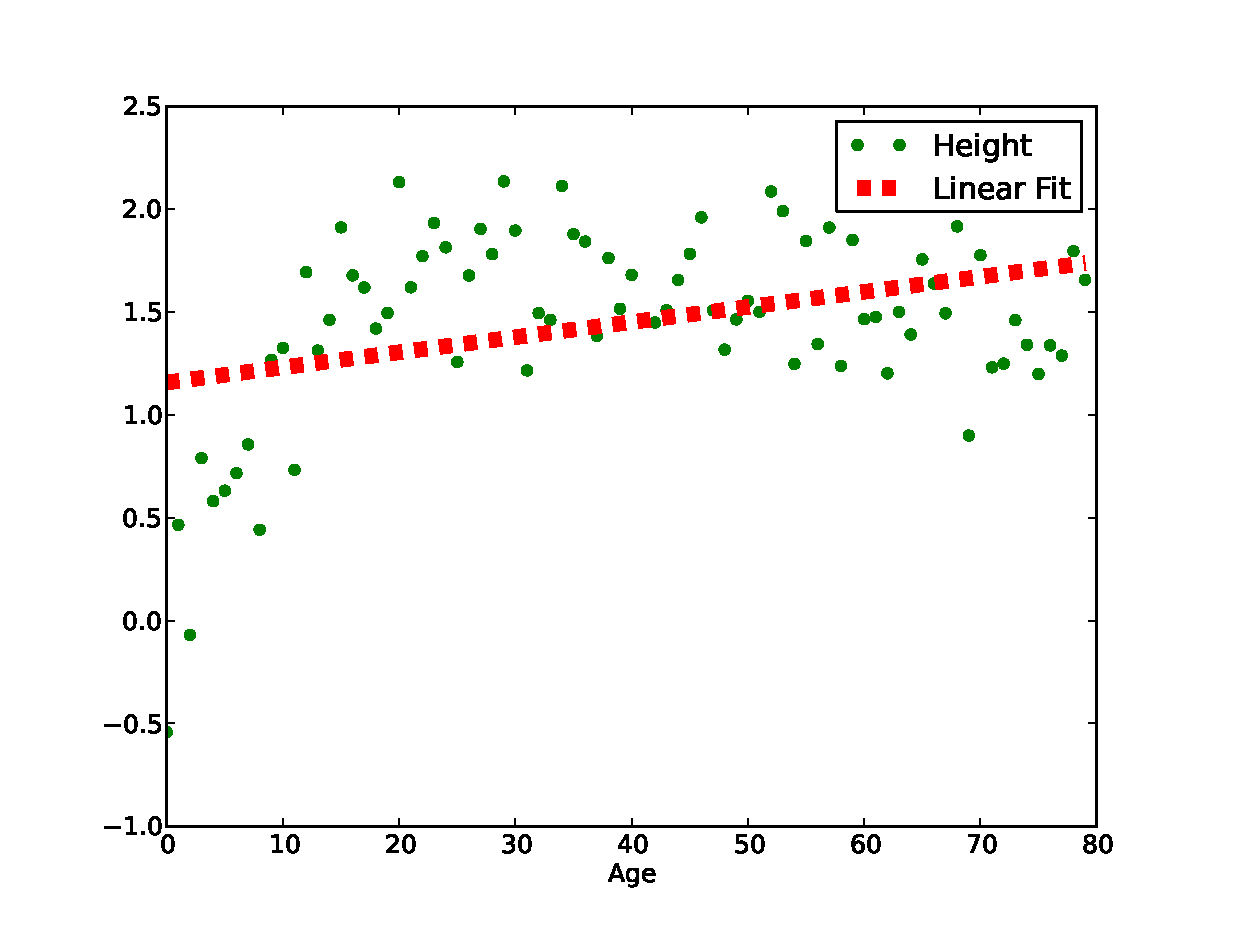
\includegraphics[width=0.5\textwidth]{../images/height_v_age_linearfit}
  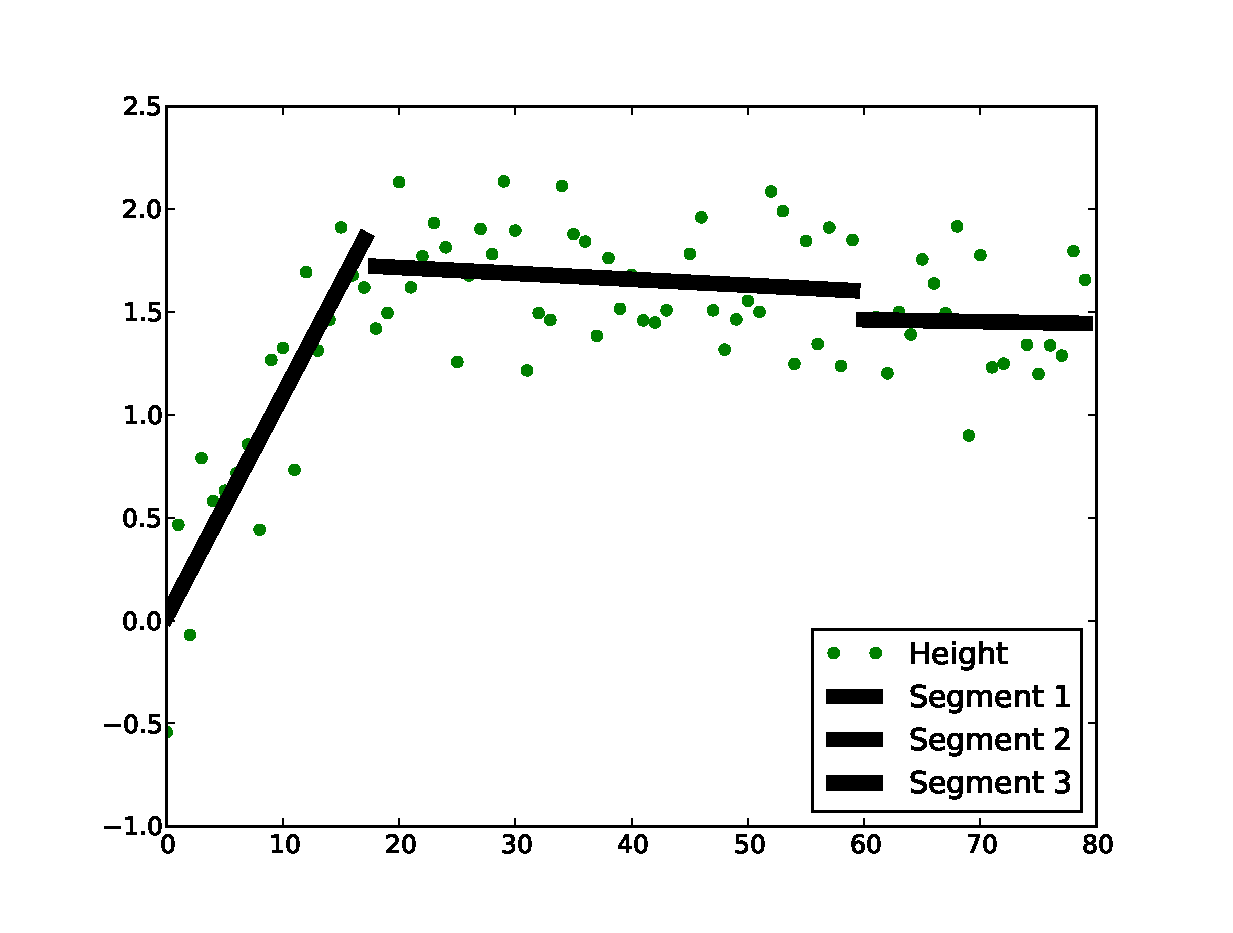
\includegraphics[width=0.5\textwidth]{../images/height_v_age_segmentfit}
  \caption{Left:  Fitting height vs. age with a linear function.  Right:  Fitting with a segmented function.  Fake data.}
\end{figure}
If we try to use height by itself, then it will have a hard time fitting this non-linear curve.  See figure \ref{linear:fig:mean-height} left.  A better alternative would be to put a nonlinear transformation of height.  Perhaps take the (sample) mean height as a function of age.  One more possibility is to \emph{segment} your model into three groups:  People between zero and eighteen, people between eighteen and sixty, and people older than sixty.  Then, three different models could be built.  Which is best?  If you are only using height, then using a mean curve would be better than segmenting, since, at best, the segments can only hope to achieve the mean.  When combined with other variables however, segmentation allows more room for the model to adjust since, e.g. the fit between eighteen and sixty won't effect the fit between zero and eighteen.  Segmenting has the disadvantage in that it requires splitting the data up into three smaller groups and keeping track of three models.

\section{Error Metrics}
To evaluate your model you need some metrics.  In our case, linear regression produces a point estimate $\hat w$.  From this it is easy to obtain a prediction $\hat Y = X\hat w$.  These can be compared in a few different ways.  Note that any method can be performed on the training set or a test/cross-validation set.

The most popular metric seems to be the \emph{coefficient of determination}, or $R^2$ (spoken as \emph{R-squared}).  This is defined as
\begin{align}
  1 - \frac{\|X\hat w - Y\|^2}{\|\bar Y- Y\|^2},
  \label{linear:align:R2}
\end{align}
where $\bar Y$ is the $N\times1$ vector with every entry equal to the mean of $Y$.  $R^2$ enjoys some nice properties, which we leave as an exercise.

\begin{exercise}
  Show that\ldots
\begin{enumerate}
  \item a perfect model ($X\hat w = Y$) will lead to $R^2=1$.
  \item if $X$, $Y$ are the training set, and $X$ contains a constant column, $0\leq R^2 \leq 1$.
  \item if $X$ does not contain a constant column, $R^2$ could in some cases be less than zero.
  \item if $X$ and $Y$ are not the training set, $R^2$ could in some cases be less than zero.
\end{enumerate}
\end{exercise}

$R^2$ has a few different interpretations.
\begin{enumerate}
  \item[(i)]  The denominator in the ratio in \eqref{linear:align:R2} can be thought of as the variability in the data.  The numerator can be thought of as the variability unexplained by the model.  Subtracting the ratio from one we get $R^2$, the \emph{fraction of variability explained by the model}.
  \item[(ii)] $R^2$ can also be thought of as \emph{the improvement from null model to the fitted model}.  We will generalize this idea later in the chapter on logistic regression.
  \item[(iii)] For linear models, $R^2$ is the \emph{square of the correlation} between the model's predicted values and the actual values.
\end{enumerate}

Since squaring a number smaller than one makes it smaller, and squaring a number larger than one makes it larger, $R^2$ will tend to penalize larger errors more.  More generally, define the \emph{L-p norm} as 
\begin{align*}
  \|X\hat w - Y\|_p :&= \left( \sum_{n=1}^N |X_{n:}\cdot \hat w - Y_{n:}|^p \right)^{1/p},
\end{align*}
and the \emph{L-infinity} norm as
\begin{align*}
  \|X\hat w - Y\|_\infty :&= \max\left\{ |X_{n:}\cdot \hat w - Y_{n:}| \right\}.
\end{align*}
If $p=1$ then we are computing ($N$ times) the \emph{mean absolute error}.

\begin{exercise}
  Show that\ldots
  \begin{enumerate}
    \item as $p\to\infty$, $\|X\hat w - Y\|_p\to \|X\hat w - Y\|_\infty$.  In other words, as $p$ increases we are penalizing the larger deviations more and more
    \item as $p\to0$, $\|X\hat w - Y\|_p$ tends to the number of elements of $X\hat w$ and $Y$ that differ.  In other words, decreasing $p$ penalizes all deviations equally.
  \end{enumerate}
\end{exercise}

\begin{exercise}
  Suppose we fit two linear regression models using two different datasets, $(X,Y)$ and $(X', Y')$.  Both data sets are the same length.  We notice that the $R-square$ error is bigger with $(X, Y)$ and the $L-2$ error is bigger with $(X', Y')$.  How can this be?
\end{exercise}


\section{End Notes}

An extensive introduction to similar material can be found in ``The elements of statistical learning'' by Hastie, Tibshirani, and Friedman\cite{HastieElements}.  The ``elements'' book covers more of the classical statistical tests (e.g. \emph{p-values}) which are important to understand since you will be asked to produce them.  Our theoretical treatment is designed to compliment this classical approach, and to prep you for the numerical problem.

For a more complete treatment of Bayesian prediction/inference, we refer the reader to the statistical text by Gelman \cite{GelmanBayesian}, and the machine-learning text by Bishop \cite{BishopPattern}.

A very theoretical treatment of regularization can be found in the book ``Regularization of Inverse Problems'' \cite{HeinzRegularization}.
